\documentclass{prettytex/ox/mmsc-special-topic}
\usepackage[european]{circuitikz}
\usepackage{menukeys}
\setlength{\headheight}{19.53pt}
\setlength{\headsep}{1.8em}
\setlength{\belowcaptionskip}{-8pt}
\setminted{fontsize=\footnotesize}
\AfterEndEnvironment{minted}{\vspace*{-0.8cm}}
\renewcommand{\operatorcolor}{black}
\usetikzlibrary{arrows.meta,calc,decorations.pathreplacing,graphs,quotes}

\newcommand{\iarronly}[1]{
  \node [currarrow, color=red, anchor=center,
    rotate=\ctikzgetdirection{#1-Iarrow}] at (#1-Ipos) {};
}
\newcommand{\varronly}[1]{
  \draw [color=blue] (#1-Vfrom) .. controls (#1-Vcont1)
  and (#1-Vcont2).. (#1-Vto) node [currarrow,
      sloped, anchor=tip, allow upside down,pos=1]{};
}
\NewDocumentCommand{\fixedvlen}{O{0.7cm} m m O{}}{
  % [semilength]{node}{label}[extra options]
  % get the center of the standard arrow
  \coordinate (#2-Vcenter) at ($(#2-Vfrom)!0.5!(#2-Vto)$);
  % draw an arrow of a fixed size around that center and on the same line
  \draw[-Triangle, #4] ($(#2-Vcenter)!#1!(#2-Vfrom)$) -- ($(#2-Vcenter)!#1!(#2-Vto)$);
  % position the label as in the normal voltages
  \node[anchor=\ctikzgetanchor{#2}{Vlab}, #4] at (#2-Vlab) {#3};
}
\tikzset{growing arrow/.style={decorate,
decoration={show path construction,
moveto code={},
lineto code={
\draw[line width=1pt,-{Stealth[width=12pt,length=12pt]}]
(\tikzinputsegmentfirst) --  (\tikzinputsegmentlast);
\fill ($ (\tikzinputsegmentlast)!6pt!0:(\tikzinputsegmentfirst) $) coordinate (aux)
($ (\tikzinputsegmentfirst)!0.5pt!90:(\tikzinputsegmentlast) $)
-- ($ (aux)!2pt!-90:(\tikzinputsegmentfirst) $)
--($ (aux)!2pt!90:(\tikzinputsegmentfirst) $)
-- ($ (\tikzinputsegmentfirst)!0.5pt!-90:(\tikzinputsegmentlast) $) ;
},
curveto code={},
closepath code={},
}}}

\providecommand{\tightlist}{%
  \setlength{\itemsep}{0pt}\setlength{\parskip}{0pt}}

\addbibresource{sources.bib}
\tikzexternalize[prefix=tikz/]

\newcommand{\topictitle}{Battery and Electric Vehicle Modelling \\ \normalsize Route Optimisation with the Battery in Mind}
\newcommand{\candidatenumber}{1072462}
\newcommand{\course}{Mathematical Modelling}

\makenoidxglossaries
\newacronym{ev}{EV}{Electric Vehicle}
\newacronym{ecm}{ECM}{Equivalent Circuit Model}
\newacronym{ode}{ODE}{Ordinary Differential Equations}
\newacronym{soc}{SoC}{State of Charge}
\newacronym{soh}{SoH}{State of Health}
\newacronym{osm}{OSM}{Open Street Map}
\newacronym{mcmc}{MCMC}{Markov Chain Monte Carlo}
\newacronym{hppc}{HPPC}{Hybrid Pulse Power Characterization}
\newacronym{rc}{RC}{Resistor Capacitor}

\title{\topictitle}
\author{Candidate \candidatenumber}
\date{\today}

\begin{document}
  \pagestyle{plain}
  \mmscSpecialHeader[casestudy]

  \begin{abstract}
    \label{abstract}
    This work will attempt to devise a mathematical model for Lithium-Ion batteries (cf. \Cref{fig:model-overview}) and, building on it, a model for an \gls{ev}.
    We implement the model, a first-order system of \glstext{ode}s, using the system solver functionality of MATLAB as well as a numerical forward integration scheme.
    We will use the implemented numerical simulator to make progress in a complex route finding problem using real-world road network data obtained from \gls{osm}.

    The first part of this report will focus on the model for a Lithium-Ion battery which was the focus of our project. The electrical behaviour was modelled through the Thevenin \gls{ecm}, in which we also considered battery aging effects. The second part is the route finding and optimisation problem in the context of \glstext{ev}s, which we approached using the $A^*$-algorithm and a \gls{mcmc} optimisation method.

    Our model was implemented in Python and MATLAB and there is a graphical user interface available with it that provides live insight into the model simulation and route-finding procedure (cf. \Cref{fig:user-interface,fig:perturbations}).
  \end{abstract}

  \begin{figure}[H]
    \centering
    \inputtikz{battery-model-overview}
    \caption{Schematic overview of the battery model introduced in this report. A current input $I(t)$ is converted into an output voltage $V(t)$ and corresponding \glsdesc{soh} $h(t)$ due to battery degradation (aging). The core part of the model is an \gls{ecm}, while aging is characterised by the capacity model.}
    \label{fig:model-overview}
  \end{figure}

  \pagebreak
  \pagestyle{normal}

  \section{Introduction}
  Clearly, electric batteries are a substantial component in various industries today and demand for them is ever-growing.
  This includes, especially, the renewable energy sector due to the unpredictability of energy supplies such as wind and solar power where short-term storage is a necessary evil.
  Similar relevance may be found in the car industry where one aims for highly (space-)efficient mobile storage of energy.
  In many countries / regions, \glstext{ev}s still lack a well-enlarged network of charging stations, for various reasons including for example, incompatibilties between charging station suppliers.
  Using methods introduced in the present report, we aim to optimise the customer experience and ecological friendliness of an \gls{ev} through a routing application that takes electric battery peculiarities and battery lifetime into account.

  In this report, we will consider how to model a Lithium-Ion battery, more specifically the Panasonic 18650PF for which there is some characteristic data available in the public domain \parencite{panasonicnums}.
  To do this, we will consider the Thevenin \gls{ecm}, which may be found in \Cref{fig:ecm}.
  The key idea here is to model the voltage output $V(t)$ given a current profile $I(t)$.
  This model not only depends on current and time, but also keeps track of internal quantities like the \gls{soc} $s \in [0, 1]$ and \gls{soh} $h \in [0, 1]$.
  It can be reduced to an \gls{ode} system, for which, using given profiles, we find parameters $R_0$, $R_1$, $C_1$ and more by a fitting procedure.
  Later on, we also considered aging effects of the battery through usage over time, which resulted in an additional differential equation in the system of \glstext{ode}s.

  Based on the model we obtained, verified and validated on new pulse test data, the next step was to apply the model to a real-world application, namely that of \gls{ev} routing.
  For this purpose, we obtain graph data of the road network of choice (users may enter localities as a text input) from \gls{osm} \parencite{osm}.
  In order to find the best route from A to B, the algorithm then performs a classical routing algorithm called $A^*$ (\emph{A-Star}) to find the (geometrically) shortest path between A and B, which may not yet be a feasible or optimal path to the destination but a good start.
  A good initial condition is all that the remaining algorithm requires, which is a Monte-Carlo iterative method that repeatedly applies small, well-defined, perturbations to the graph route and then obtains a time or cost estimate of the modified trip using the battery (and car) model we introduced.
  If the modified route yields an improvement in the metric of choice, it is accepted as the new state and the process repeats until a satisfactory route was found.

  This report will focus on explicit formulation of the problem and model, numerical simulation of an electric car on a given real-world route and path optimisation through the Metropolis-Hastings method.

  \section{Problem and Model Formulation}
  \subsection{The Isolated Battery}
  In order to model a Lithium-Ion battery in and of itself, we consider the following (physical) quantities:
  Let
  $s \in [0, 1]$ denote the \glsdesc{soc} of the battery,
  $h \in [0, 1]$ the \glsdesc{soh},
  $Q \in \R^+$ the charge,
  $Q_{00} \in \R^+$ the maximum possible charge at the time of production (\textcolor{gray}{in Coulombs}),
  $V \in \R$ the voltage across the battery (\textcolor{gray}{in Volts}) with
  $I \in \R$ the corresponding current (\textcolor{gray}{in Amperes}) where $I > 0$ corresponds to discharging the battery.
  Then, per common definition, $s := \frac{Q}{Q_0}$ is the amount of charge currently present in the battery as compared to $Q_0 \in \R^+$ the current maximum capacity, which itself is dependent on the \gls{soh}, as given by $Q_0 := h Q_{00}$.
  Further let
  $T \in [-273.15, \infty)$ denote the temperature of the battery (\textcolor{gray}{in degrees Celsius}) and
  let $t \in \R$ represent time (\textcolor{gray}{in seconds}).
  Let $c \in \R^+$ denote the cycle, so the number of full discharges of the battery.

  From the definition of current $I := \frac{\dd Q}{\ddt}$, we further have that for a single cycle,
  $$s(t) = \frac{Q(t)}{Q_0} = 1 - \frac{1}{Q_0} \int_0^t I(\tau) \,\dd\tau \,,$$
  under the assumption that $Q_0$, and therefore $h$, stays constant during that cycle.

  \subsection{The Equivalent Circuit Model}
  As mentioned earlier, we want to model the battery as an electrical component which exerts specific behaviour in an electrical circuit.
  In electrical engineering, such models of more complicated components are frequently represented by equivalent circuits which only consist of basic components, mostly resistors, diodes, transistors, capacitors and inductors.

  \begin{figure}[H]
    \centering
    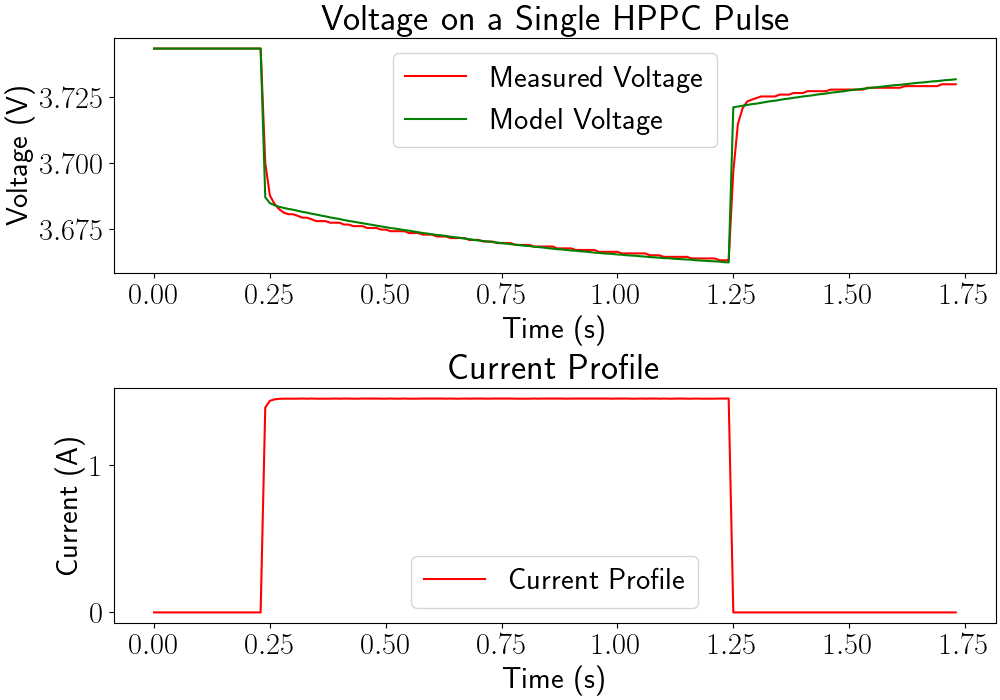
\includegraphics[width=0.6\linewidth]{figures/hppc-pulse.png}
    \caption{One of the sample \gls{hppc} pulses we used for parameter finding. We want to model the output voltage $V(t)$ given a current input profile $I(t)$. Each sample is characterised at a specific \glsdesc{soc} $s$, \glsdesc{soh} $h$ and temperature $T$, this one was taken at $s \approx 1$, $h \approx 1$ and $T = \SI{10}{\degreeCelsius}$.}
    \label{fig:hppc-pulse}
  \end{figure}

  Empirically, we know that a battery's voltage output for a current pulse looks roughly as given in \Cref{fig:hppc-pulse}, which is part of a standardised cycle characterisation procedure taking the battery from ``fully charged'' ($s=1$) to ``completely empty'' ($s=0$). Data is due to \cite{panasonicnums}.
  As one can see from the voltage curve, the battery exerts a ``time-relaxation'' behaviour on high-frequency changes in the current.
  One way of modelling this is through an \glstext{rc} circuit, confer \Cref{fig:ecm}: the parallel circuit of $R_1$ and $C_1$ is responsible for the exponentially decaying behaviour in the voltage curve given (near-)jumps in the current.
  Additional ohmic impedance is modelled through $R_0$.
  The ``heart'' of the \gls{ecm} is the open-circuit voltage $V_{OC}$ which behaves like a voltage source but strongly depends on parameters $s$, $h$ and $T$.
  We modelled it accordingly, using a polynomial ansatz including cross-terms $$V_{OC}(s, h, T) = c_1 s + c_2 h + c_3 T + c_4 sh + c_5 sT + c_6 hT + c_7 shT + \mathcal{O}(s^2, h^2, T^2, ...)\,,$$
  and similar polynomials are chosen for $R_0$, $R_1$ and $C_1$, completing the model.
  Using the abovementioned dataset \parencite{panasonicnums}, these fits were obtained numerically using a least-squares fitting procedure. An example of the dependency on the \gls{soc} can be found in \Cref{fig:parameters}.

  \begin{figure}[H]
    \centering
    \inputtikz{ecm-model}
    \caption{
      The Thevenin \gls{ecm} with parameters $R_0 \in \R^+$, $R_1 \in \R^+$ and $C_1 \in \R^+$ and $V_{\rm OC} \in \R^+$ the \textit{open circuit voltage} which behaves according to a function $V_{\rm OC}(s, h, T)$ dependent on $s$, $h$ and $T$.
    }
    \label{fig:ecm}
  \end{figure}

  Kirchhoff's law then tells us that the currents $I_{R1} \in \R$ and $I_{C1} \in \R$ add up to the total current $I = I_{R1} + I_{C1}$, and that the voltages $V_0, V_1 \in \R$ and $V_{\rm OC}$ sum up to $V = V_0 + V_1 + V_{\rm OC}$.
  The capacitor behaves according to $I_{C1} = C_1 \frac{\dd V_1}{\ddt}$, while the resistors follow Ohm's law $V_0 = R_0 I$ and $V_1 = R_1 I_{R1}$.
  The resulting circuit then behaves approximately as a real Lithium-Ion battery would in many relevant situations.

  \begin{figure}[H]
    \captionsetup[subfigure]{justification=centering}
    \centering
    \subfloat[Fit of $R_0$ as a function of the \gls{soc} ($s$).]{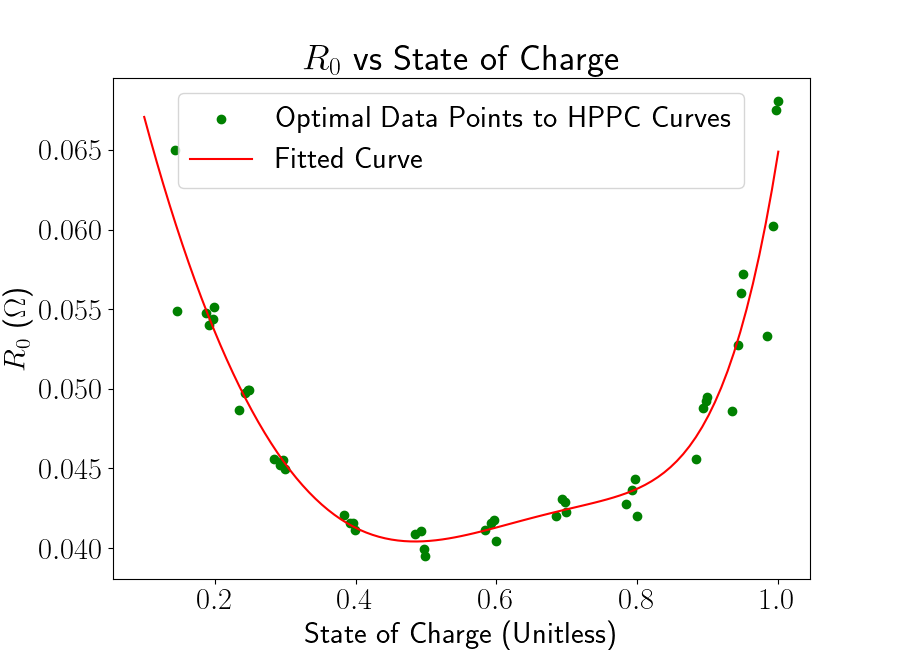
\includegraphics[width=.5\linewidth]{figures/r0fit.png}}\hfill
    \subfloat[Fit of $R_1$ as a function of the \gls{soc} ($s$).]{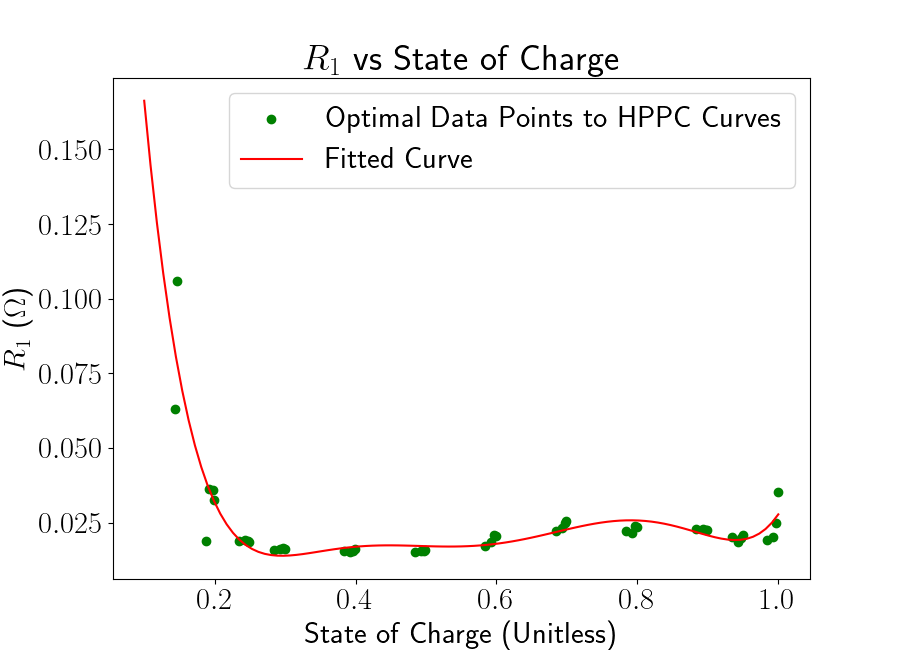
\includegraphics[width=.5\linewidth]{figures/r1fit.png}}\par
    \caption{Dependencies of the Thevenin equivalent circuit (\Cref{fig:ecm}) model's parameters $R_0$ and $R_1$ on the \gls{soc} with a polynomial fit through the data points. Data is again due to \cite{panasonicnums}.}
    \label{fig:parameters}
  \end{figure}

  Let us consider an application of this model in an \glsdesc{ev} next.

  \subsection{Battery in an Electric Vehicle}
  In order to model a road network, let us first consider the definition of an undirected graph $G = (V_G, E)$. We take an undirected graph for simplicity, assuming that cars may go in arbitrary direction along each edge.
  \begin{definition}{Undirected Graph}{undirected-graph}
    A graph $G = (V_G, E)$ with vertices $V_G$ and edges $E \subseteq V_G \times V_G$ is undirected if and only if $(v_i, v_j) \in E \Rightarrow (v_j, v_i) \in E \quad \forall\; v_i, v_j \in V_G$.
  \end{definition}

  Modelling a vehicle on a road network requires a few more definitions.
  On a graph $(V_G, E)$ with edges $E = \{AB, AC, ...\} \subseteq V_G \times V_G$ and vertices $V_G = \{A, B, ...\}$, let
  $d_{AB} \in \R^+$ denote the distance between two vertices $A \in V_G$ and $B \in V_G$ (\textcolor{gray}{in meters}),
  $x = x_{AB} \in [0, d_{AB}]$ the progress (current location) on the route from vertex $A$ to $B$ (\textcolor{gray}{in meters}),
  $v := \frac{\ddx}{\ddt}$ denote the current velocity with
  $v_{\rm max, AB} \in \R^+$ the maximum allowed velocity on $AB$ (\textcolor{gray}{in meters per second}).
  Then let
  $T_{\rm env}(x) \in [-273.15, \infty)$ denote the temperature of the environment (\textcolor{gray}{in degrees Celsius}) at location $x$.
  Note that this graph-based approach to the problem does not require any more geometric information about the network than edge lengths $\{d_{ij}\}_{i,j}$, while it may of course be motivated by spherical coordinates on the earth.
  Consider for example \Cref{fig:graz-to-munich} or \Cref{fig:grannys-stations} for an actual route in Ireland.

  \begin{figure}[H]
    \centering
    \inputtikz{graz-to-munich}
    \caption{Exemplary route from Graz to Munich on a road network $(V_G, E)$, where edge weights correspond to distances in between the physical places represented by nodes.}
    \label{fig:graz-to-munich}
  \end{figure}

  The model of our car still lacks a component realising electrical into mechanical power (a motor).
  Let $P \in \R$, $P := I \cdot V$ denote the (electrical) power the car draws from the battery (\textcolor{gray}{in Watts}) so $P > 0$ corresponds to discharging the battery.
  This power is to be realised into a mechanical component $P_{\rm motor} \in \R^+$ driving the car forwards, heating for the battery $P_{\rm heat} \in \R^+$, $P_{\rm heat} = c (T - T_{\rm env})$, with $c \in \R^+$ the heat conduction constant describing the relation between the heater and battery, and power dissipation $P_{\rm diss} \in \R^+$.
  While driving, $P = P_{\rm motor} + P_{\rm heat} + P_{\rm diss}$.
  The acceleration of the car $a \in \R$ (\textcolor{gray}{in meters per second squared}), where $a := \frac{\dd v}{\ddt} = \frac{\dd^2 x}{\ddt}$ is decomposed into $a_m \in \R$, which directly impacts $P_{\rm motor}(a_m)$, and the deceleration due to friction (air, etc.) $a_f(v) \in \R^-$, so that in total $a = a_m + a_f$.

  Most electric cars have a range from approximately 160 up to 650 km \parencite{range}, making route changes through charging stations a necessity for longer trips.
  The resulting routing problem we want to solve then inspires the following definitions of charging stations.
  On the graph $(V_G, E)$ there exists a set of EV charging stations $V_{\rm charge} \subseteq V_G$ where $P_{C,\rm charge}$ denotes the possible charging power (\textcolor{gray}{in Watts}) at the charging station vertex $C \in V_{\rm charge}$ with $K_C \in \R^+$ the occuring costs per energy unit (\textcolor{gray}{in Euros per Watt second}) and $t_C \in \R^+$ the charging time per charging station (time spent at the charger, \textcolor{gray}{in seconds})\footnote{
    Charging station \& street data was obtained from \href{https://osm.org/}{OpenStreetMap} and subsequently invoking
    \texttt{osmfilter england-latest.o5m \-\-keep="amenity=charging\_station"}.
    Daily dumps of \gls{osm}'s public map data were obtained from \url{https://download.geofabrik.de/}.
  }.

  \subsection{Battery Degradation (Aging)}
  A central aspect considered in our project was to study the effects of battery degredation, or aging.
  In this context, cycle aging (a short-term effect) is frequently distinguished from calendar aging (a long-term effect).
  One possible model for this would be to express $Q_0$ in terms of the original capacity at the time of production $Q_{00}$ along with multiple degradation effects that we consider:
  \begin{equation}
    \label{eq:cap}
    Q_0(t,c,s,I) = Q_{00} - \frac{F_{\rm acycle}(c)}{F_{\rm current}(I)} - F_{\rm cal} \quad \in [0, Q_{00}]\,.
  \end{equation}
  By $F_{\rm acycle}(c) \in \R$ we denote the \textbf{Current Agnostic Cycle Degradation Factor} which models cycle aging at a single current. It models the aging effects resulting only from discharge usage of the battery, at an idealised single current.
  $F_{\rm current}(I) \in (0, 1]$ represents the \textbf{Current Scaling Factor}, a value that incorporates behaviour where higher currents are worse for cycle aging \parencite{csfpaper}. This term is highly relevant for scenarios where one can choose the amount of current drawn from the battery and then optimise accordingly if this behaviour is well-known.
  Finally, $F_{\rm cal}(s,t) \in \R$, the \textbf{Calendar Degradation Factor}, ages the battery over time and accounts for suboptimal storage in terms of the \gls{soc}.
  Storage at the right \gls{soc} and environment is one of the most crucial aspects for battery lifetime.

  The \glsdesc{soh} $h$, the ratio between $Q_0$ and $Q_{00}$ is then given by
  $$h = \frac{Q_0}{Q_{00}} = 1 - \frac{F_{\rm acycle}(c) + F_{\rm cal} F_{\rm current}(I)}{F_{\rm current}(I) Q_{00}} \quad \in [0, 1]\,,$$
  directly following from \Cref{eq:cap} and yielding a simple, yet effective approximation for aging of the battery.
  Experimental data suggests a ``knee-bending'' behaviour towards the end of a battery's lifetime, which motivated the following expressions.
  In our model, we used
  \begin{align*}
    F_{\rm acycle}  & = c \left( \alpha_1 + \alpha_2 \exp{\alpha_3c-\alpha_4} \right)\,,                                                                                                                     \\
    F_{\rm current} & = \alpha_5 - \alpha_6 \exp{ \alpha_7 I - \alpha_8}\,,                                                                                                                                  \\
    F_{\rm cal}     & = \int \left( \alpha_9(T) \left\{\cosh({\alpha_{10}s - \alpha_{11}}) + \alpha_{10} t \, \abs{\sinh({\alpha_{10} s- \alpha_{11}})} \, \abs{ \frac{\dds}{\ddt}}\right\}\right) \,\ddt\,,
  \end{align*}
  in part following \cite{csfpaper}, but largely our own work
  with $\alpha_{1, ..., 11} \in \R$ various parameters obtained through least-squares fitting procedures.
  A plot of the degredation function is given in \Cref{fig:aging}, using the given expressions for $F_{\rm acycle}$, $F_{\rm current}$ and $F_{\rm cal}$.

  \begin{figure}[H]
    \centering
    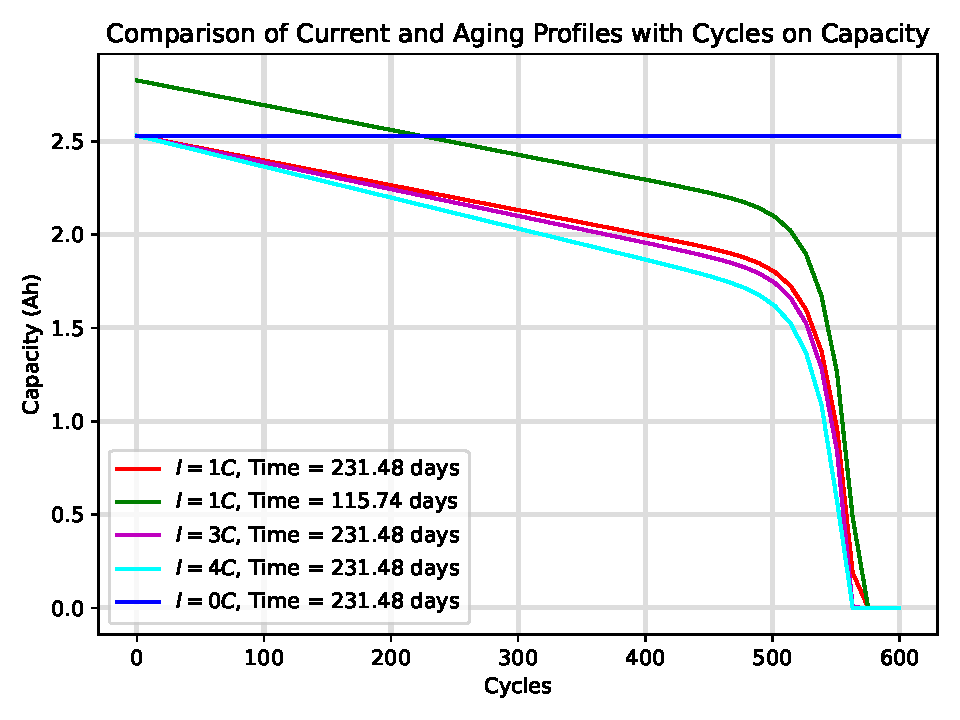
\includegraphics[width=0.7\linewidth]{figures/aging.pdf}
    \caption{Capacity over discharging cycles behaviour according to the degradation model of the battery, according to \Cref{eq:cap} with $Q_{00} = \SI{2.9}{\ampere\hour}$. Each line corresponds to different discharge currents $I$, as multiples of the capacity, and a different battery aging time.}
    \label{fig:aging}
  \end{figure}

  Using the car and road network models introduced above, in general terms the problem may be stated as follows:

  \subsection{A Variational Optimisation Problem}
  \label{sec:problem}
  Given source and destination vertices $A, Z \in V_G$ on the graph $(V_G, E)$, \textbf{which connected set of edges} $E_R \subseteq E$ connecting $A$ to $Z$, set of visited \textbf{charging stations} $V_C \subseteq V_{\rm charge}$ along $E_R$ and \textbf{charging times} $\{t_C\}_{C \in V_C}$ visited on the route $E_R$, and \textbf{driving behaviour} $a_m(x, v, t, s, h, T_{\rm env}, ...),\, a_m \in \cC^1(\P)$ with $\P$ the parameter space, \textbf{minimises}
  \begin{enumerate}
    \item the total travel time $t_{\rm total} := \int_{E_R} \frac{1}{v} \,\ddx + \sum_{C \in V_C} t_C$, where we assume that turning takes no additional time,
    \item the total cost of travel $K := \sum_{C \in V_C} P_{C, \rm charge} t_{C} K_C$,
    \item or $-N$ where $N$ is the highest possible number of repetitions (commutes from $A$ to $Z$) with the same battery (requiring $h > 0$). \label{minoption:aging}
  \end{enumerate}
  In other words, we aim to minimise the functional $F \in \cC(\P)^*$, so $F: \cC(\P) \mapsto \R$ where either $F[a_m, E_R, V_C, t_C] = t_{\rm total}$, $F[a_m, E_R, V_C, t_C] = K$ or $F[a_m, E_R, V_C, t_C] = -N$.

  Obviously, solving the stated problem in its full form and with all the given details is a task exceeding the scope of this project, although we were able to make some progress in the direction of it.
  The intention here is to state the model in high generality and be clear about the simplifications that were made within the scope of this report in order to be able to move ahead.

  There are endless possibilities to simplify, for example one could take
  $V_G = \{A, B\}$ and $E = \{AB\}$ with some $d_{AB}$, $v_{\rm max, AB} = \infty$ and $V_C = \{\}$, so only looking at the minimisation of $t_{\rm total}$. This is equivalent to ignoring the graph-algorithmic component of the problem, as it is only a single line without a charger.
  Another potential simplifcation would be to take $h = 1$ to ignore battery aging / degradation effects. Or even more radically, $s = \rm const.$ to only model extremely short-term (on the order of seconds) effects of this model.

  In the remaining sections of the report, we will assume the following:
  \begin{itemize}
    \tightlist
    \item $T = T_{\rm env} = \rm const. = \SI{10}{\degreeCelsius}$ and therefore $P_{\rm heat} = 0$ to ignore the motor heating component. We neglected temperature changes in the environment and a respective battery heating strategy $P_{\rm heat}(x, v, t, s, h, T_{\rm env}, ...)$, $P_{\rm heat} \in \cC(\P)$.
    \item $P_{\rm diss} = 0$ as this is an easily implementable extension to the existing model.
    \item $v_{{\rm max}, ij} = \infty \,\forall\, i, j$ so there is no speed limit, although data is potentially available.
  \end{itemize}

  \section{Numerical Simulation of a Car}
  \label{sec:simulator}
  Now that the model is defined, it remains to be implemented.
  The resulting \gls{ode} system can be solved using an available \gls{ode} system solver such as \texttt{ode15s} in MATLAB.
  While this is the more accurate approach, it is harder to generalise it to a graph where environmental conditions change along different edges of the network.
  Nevertheless, given the problem settings, it is well possible.
  We will however not focus on it within the scope of this report.
  Our solver uses a simple Forward Euler discretisation.

  For a first-order (nonlinear) \gls{ode} system $\dot{\vec{x}} = \vec{f}(\vec{x})$, a solution may be approximated by the Forward Euler scheme
  \begin{equation}
    \frac{1}{\Delta t} \left(\vec{x}_{n+1} - \vec{x}_{n}\right) = \vec{f}(\vec{x}_n), \quad \text{ so } \quad \vec{x}_{n+1} = \vec{x}_{n} + \Delta t \cdot \vec{f}(\vec{x}_n)\,,
    \label{eq:forward-euler}
  \end{equation}
  to get the approximant $\vec{x}^n$ at the $n$-th timestep with parameter $\Delta t$ and some initial condition $\vec{x}_{0}$.
  Our code used this scheme to solve the \gls{ode} system resulting from the \gls{ecm}. More information on the code can be found in \Cref{sec:code}.
  Along with the numerical simulator and optimiser, we implemented a graphical user interface (cf. \Cref{fig:user-interface}) for the problem, capable of loading any graph.

  \begin{figure}[H]
    \centering
    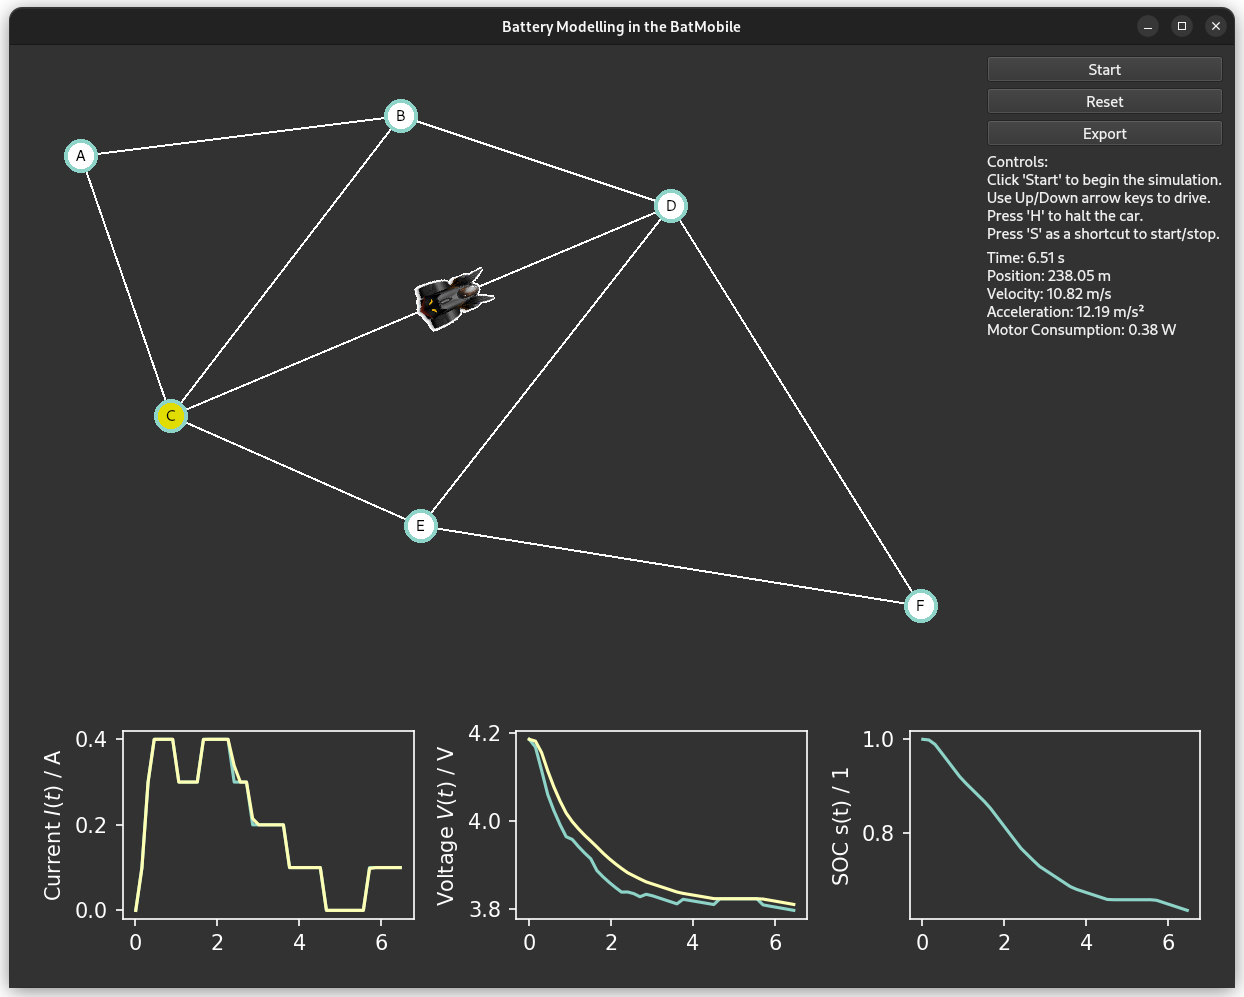
\includegraphics[width=0.65\linewidth]{figures/screenshot.png}
    \caption{Screenshot of the Qt6 user interface of the car simulation software accompanying this report (confer \Cref{sec:code}) running on the graph depicted in \Cref{fig:graz-to-munich}. Using the arrow keys, one can control the battery mobile (\textit{batmobile}) along edges of the road network.}
    \label{fig:user-interface}
  \end{figure}

  Pressing \keys{$\uparrow$} accelerates the car and the resulting battery model changes can be observed in real-time using the charts at the bottom. \keys{$\downarrow$} decelerates (in this scenario, we used current-control, so $I(t)$ is decreased).

  The simulator then iteratively updates the state $\vec{x}^n$ comprised of position $x$, velocity $v$, acceleration $a$, \glsdesc{soc} $s$, currents $I$ and $I_{R1}$, voltage $V$, current edge $(v_i, v_j) \in E$ to name the most central components, in time using \Cref{eq:forward-euler}.
  In the implementation, we assume that power output $P = IV$ of the battery is directly proportional to mechanical acceleration $a_m$ using a factor.
  We model friction by
  $$a_f = a_{\rm drag} v^2 + a_{\rm friction}\,,\quad a_{\rm drag}, a_{\rm friction} \in \R^-\,,$$
  which then results in $a = a_m + a_f$.
  Integrating results in velocity and position.

  Next up, we will consider the route finding approach and optimisation procedure.

  \section{Metropolis-Hastings and A-Star}
  As mentioned in the introduction, our algorithm consists of two main parts.
  The first step is to find the geometrically shortest path using the $A^*$-algorithm from computer science.
  The second step is to perturb this path in a \gls{mcmc} optimisation routine that also takes the battery model into account, and finds good driving behaviour along a perturbed route $E_R$ along charging stations $V_C$.

  In order to find good / optimal driving behaviour $a_m$ along the route, we consider the following function basis expansion:
  \begin{equation}
    a_m^{(i,j)}(x, s, t) = \sum_{k=0}^{n} a_{k,1}^{(i,j)} T_k(x) + a_{k,2}^{(i,j)} T_k(s) + a_{k,3} T_k(t)\,, \text{ per edge } (v_i, v_j) \in E_R\,,
    \label{eq:spectral-expansion}
  \end{equation}
  where $\{T_k\}_{k\in \N_0}$ may be any function basis, for instance the Chebyshev polynomials defined by $T_k(\cos \theta) = \cos(k\theta)$.
  We assume that the driving behaviour along an edge does not need to be complex in order to be effective, so low expansion orders might suffice for a relatively good result (e.g. $n = 1, 2, 3$).
  The problem of finding the optimal driving behaviour is then reduced to finding the coefficients $\left\{a_{k,\{1,2,3\}}^{(i,j)}\right\}_{k\in\N_0}$ which is already much more straightforward than minimising a functional.
  An approach of this form can generally be regarded as a spectral method.

  \subsection{Shortest Path Finding}
  As a first step, we aim to find a good initial condition to the \gls{mcmc} route optimisation routine.
  This is the shortest path, which we will find using the $A^*$ (A-Star) search algorithm.

  The graph data was retrieved using OSMnx \parencite{osmnx} which itself is built on top of NetworkX \parencite{networkx}. The edges retrieved from the \glsdesc{osm} API also contain data on the highest allowed velocity $v_{\rm max}$, but we did not use it in our solver as this would need to be a carefully considered constraint to the optimisation routine.

  $A^*$ is based on Dijkstra's algorithm which is already highly efficient for any graph but can be made even more effective by incorporating a distance heuristic into the algorithm.
  This distance heuristic, for our purposes of a road network, is given by the airline distance between two vertices $v_i$ and $v_j \in V_G$.
  In general, it could be any mapping $H: V_G \times V_G \mapsto \R^+$ that roughly approximates the true shortest path length between $v_i$ and $v_j$ \parencite{astar}.

  The $A^*$ algorithm then leverages this distance heuristic in order to not need to search through all vertices (as Dijkstra's algorithm would) but only a subset of them which are in the direction of the target node.
  This facilitates an incredible speedup on street networks which are normally huge.

  \begin{algorithm}[language=pseudo,basicstyle=\footnotesize,caption={\centering The $A^*$-search algorithm \parencite{astar}}]
open_list, closed_list = empty list of possible positions
adjacent_val = 0
next_position = null
push start_position to open_list
while open_list is not empty, do
  current_node = pop(open_list)
  for each adjacent position of current_node (ap_current)
        with value (av_current), do
    if (adjacent_val < av_current) or (ap_current $\in$ closed_list), do
      adjacent_val = av_current
      next_position = ap_current
    push ap_current to closed_list
  push next_position to open_list
  \end{algorithm}

  The truly magical aspect of this algorithm is that in the context of a geometric network, it still returns \textit{the} optimal shortest path in between two vertices, despite taking much less runtime than Dijkstra's algorithm \parencite{astar}.
  For the optimiser accompanying this report, we used NetworkX's implementation of $A^*$.

  \subsection{Monte-Carlo Optimisation}
  With this initial route in mind, we will consider small perturbations to each route $E_R$.
  The state space we are optimising in here is vast, motivating the use of a Monte-Carlo method.
  So for our purposes here, we use the Metropolis-Hastings \gls{mcmc} method due to \cite{metropolis} and \cite{hastings}.

  The algorithm can then be outlined as follows, with $F^{n}$ the metric we are optimising for, for instance the total travel time $F^n = t_{\rm total} := \int_{E_R^n} \frac{1}{v} \,\ddx + \sum_{C \in V_C^n} t_C$.
  \begin{algorithm}[language=pseudo,caption={\centering The Metropolis-Hastings algorithm \parencite{metropolis, hastings}},basicstyle=\footnotesize]
until convergence, repeat
  sample a candidate $\vec{x}^*$.
  set $\vec{x}^{n+1} = \vec{x}^*$ with acceptance probability
    $p_{\rm accept} = \min\left(1, \e^{-\beta (F^{n+1} - F^n)}\right)\,,$ with $\beta \in \R^+$ a transition factor.
  Otherwise, let $\vec{x}^{n+1} = \vec{x}^{n}$.
  \end{algorithm}

  In order to sample a route candidate $\vec{x}^*$, we take the old route $E_R^n$ and perturb it to get $E_R^*$.
  We define four types of perturbations: Type-1 which turns one edge into two (taking a small detour with a connected vertex). So the route length increases.
  Type-2 which replaces a node by an adjacent node that still connects the two neighbouring vertices. The route length stays the same.
  Type-3 is a special case where the destination becomes a part of the perturbation which shortens the route to this node.
  Finally, Type-4 was added to allow for much larger changes using a NetworkX subroutine yielding a simple path between two vertices which were neighbours in the previous route. Consider for example \Cref{fig:perturbations}.

  The key idea here is to perturb charging stations in- and out of the route and compare results after performing the numerical simulation described in \Cref{sec:simulator}.
  This simulation done at every \gls{mcmc} iteration is generally highly expensive, but experiments showed that we can use a fairly large time-step $\Delta t$, therefore speeding up the simulation by a significant amount without sacrificing all too much accuracy.

  So the Monte-Carlo method explores the state-space to some extent, and returns the best route!
  Not only that, the optimal driving strategy $a_m$ can be found by incorporating the coefficients $\left\{a_{k,\{1,2,3\}}^{(i,j)}\right\}_{k\in\N_0}$ into the Monte-Carlo state variable $\vec{x}^{n}$ and perturbing these by sampling from a probability distribution.
  Because this is an iterative optimisation method, larger scales / maps (e.g. England) are not a problem! The Mathematical Institute's Linux machines are capable of handling a route between Cavan and Dublin (in Ireland) within half an hour of running time and return a reasonable result.
  Of course that is still far from optimal for a routing application where customers are used to running times below a second.
  The code is written in Python and therefore not as fast as it could be, but more remarkable performance gains can be made by further extensions and improvements to the method itself, as briefly discussed in \Cref{sec:discussion}.

  \subsection{Special Case: Granny's House}
  From a more analytical rather than numerical / simulative perspective, we considered the ``Granny's House problem'' (cf. \Cref{fig:grannys-idealised-problem-setting,fig:grannys-stations}).
  For such a simple graph, many results can be derived much more directly but they will not be presented here.
  Especially battery degradation (aging) can be much better considered in this simple setting, where we found that for young batteries it is best to run them at a high \gls{soc} and store at a moderate charge. Similarly, for old batteries it is best to avoid usage close to the extremes $s = 0$ and $s = 1$.

  \begin{figure}[H]
    \centering
    \inputtikz{grannys-house}
    \caption{The graph of our exemplary problem ``Granny's House'', a simplified case of the problem described in \Cref{sec:problem}. The situation is that we want to visit our grandmother, who lives \SI{115}{\kilo\meter} away from our home, in regular intervals. Along the route, there are two chargers. Our car only has a range of \SI{200}{\kilo\meter}. Is it better to charge at the first or second charger, on the way there or on the way back?}
    \label{fig:grannys-idealised-problem-setting}
  \end{figure}

  \begin{figure}[H]
    \centering
    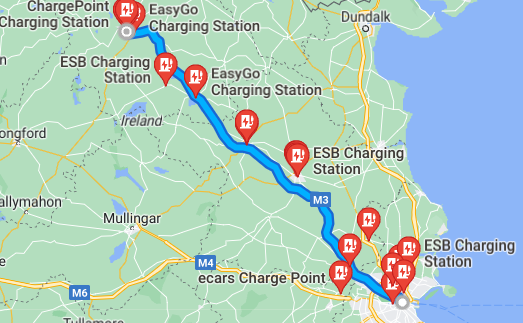
\includegraphics[width=0.4\linewidth]{figures/grannys-stations.png}
    \caption{The unperturbed route for the ``Granny's House'' problem in Ireland from Dublin to Cavan, with charging stations depicted using red pins \parencite{googlemaps}.}
    \label{fig:grannys-stations}
  \end{figure}

  \subsection{Special Case: Routing in Jericho}
  \begin{figure}[H]
    \centering
    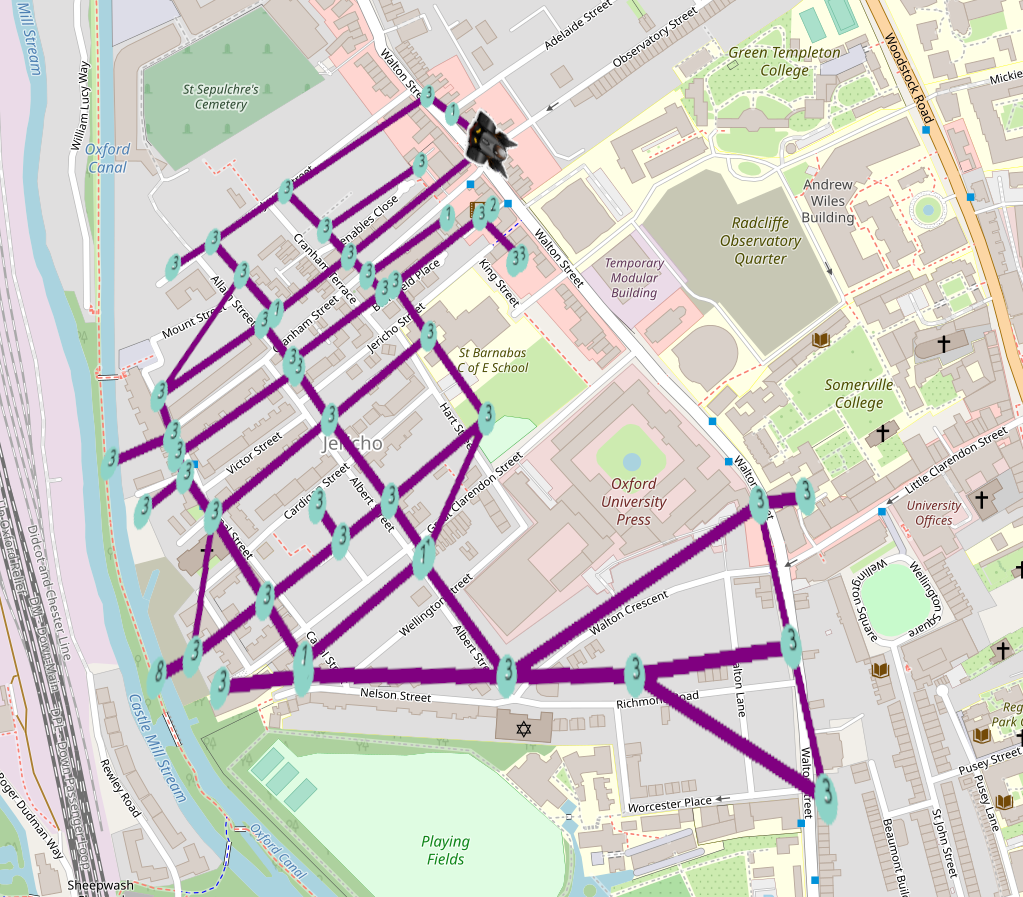
\includegraphics[width=0.45\linewidth]{figures/jericho.png}
    \caption{Overlay of the routing graph on a map of Jericho, Oxford, Oxfordshire \parencite{osm}, without adjusting for the Merkator projection or non-linear roads, which leads to a slightly skewed appearance. The Mathematical Institute is adjacent to one of the shown edges.}
    \label{fig:jericho}
  \end{figure}

  \begin{figure}[H]
    \captionsetup[subfigure]{justification=centering}
    \centering
    \subfloat[Original route as returned by $A^*$.]{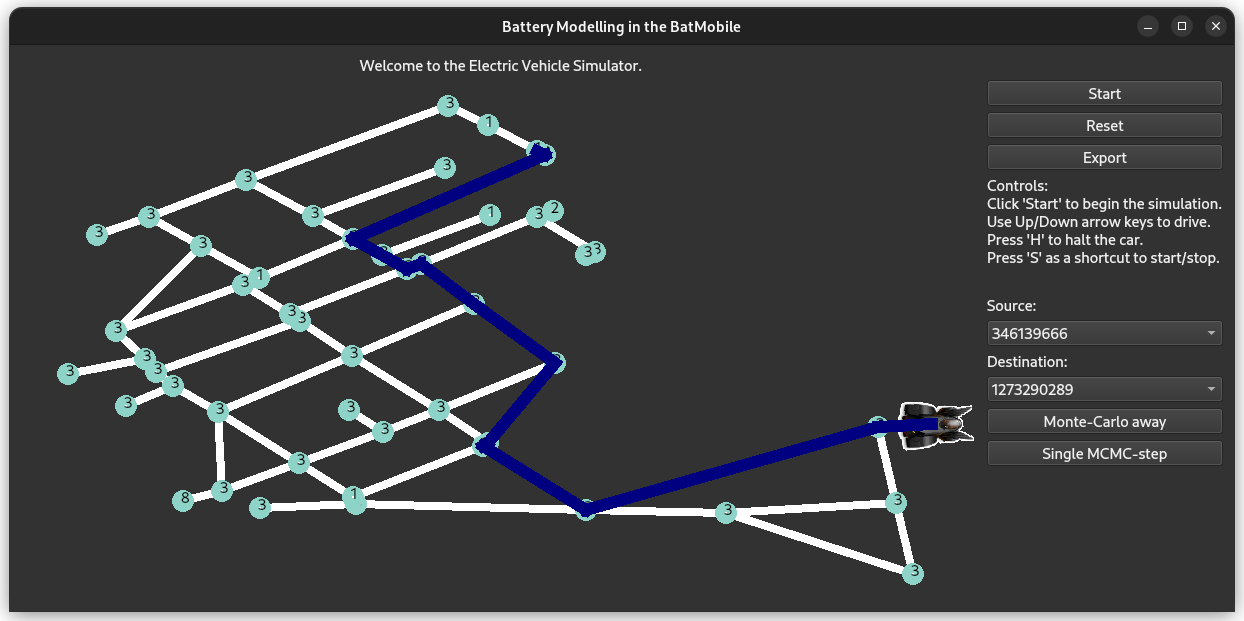
\includegraphics[width=.5\linewidth]{figures/route1.png}}\hfill
    \subfloat[Perturbed route.]{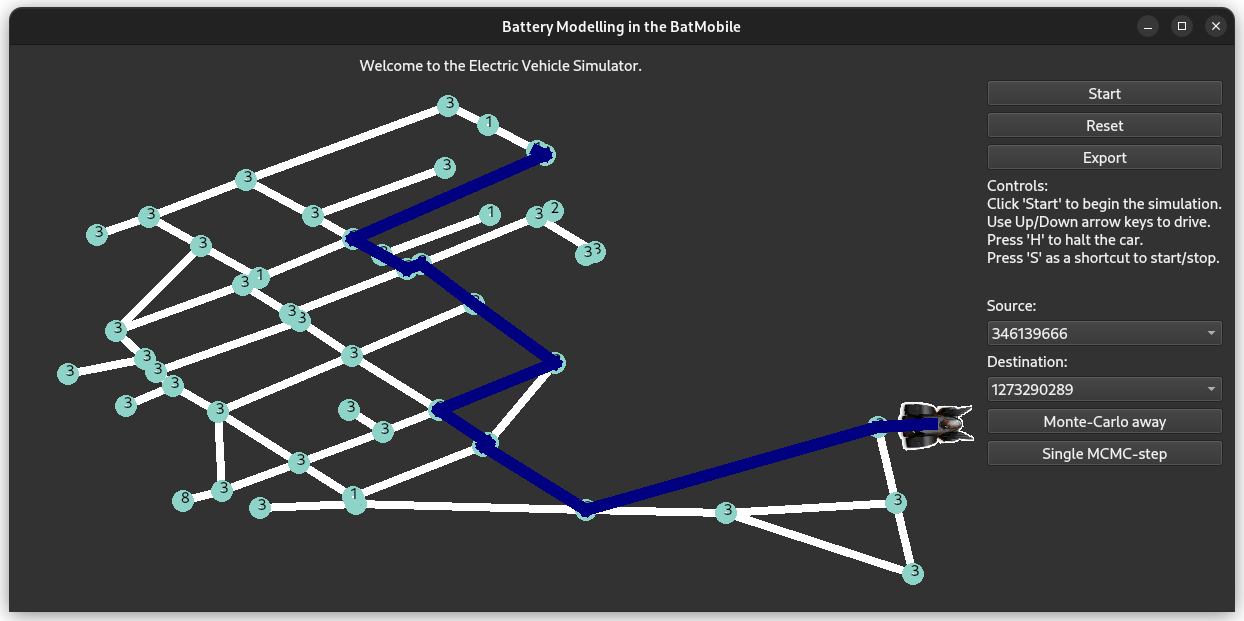
\includegraphics[width=.5\linewidth]{figures/route2.png}}\par
    \vspace{0.5cm}
    \subfloat[Perturbed route.]{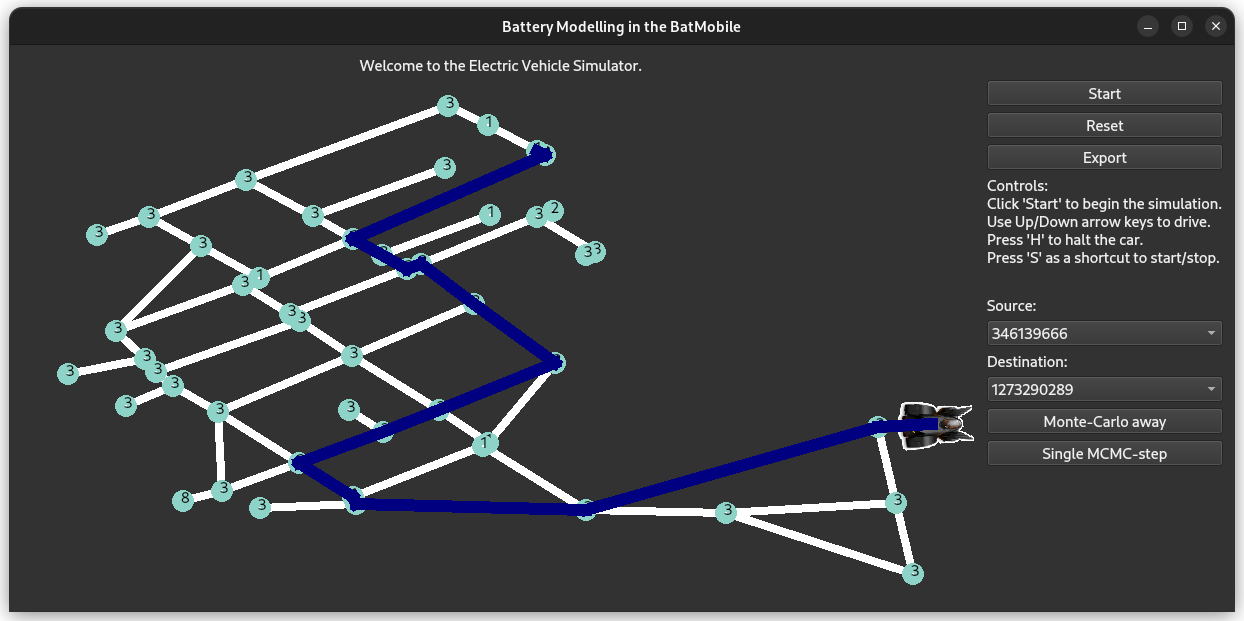
\includegraphics[width=.5\linewidth]{figures/route3.png}}\hfill
    \subfloat[Perturbed route.]{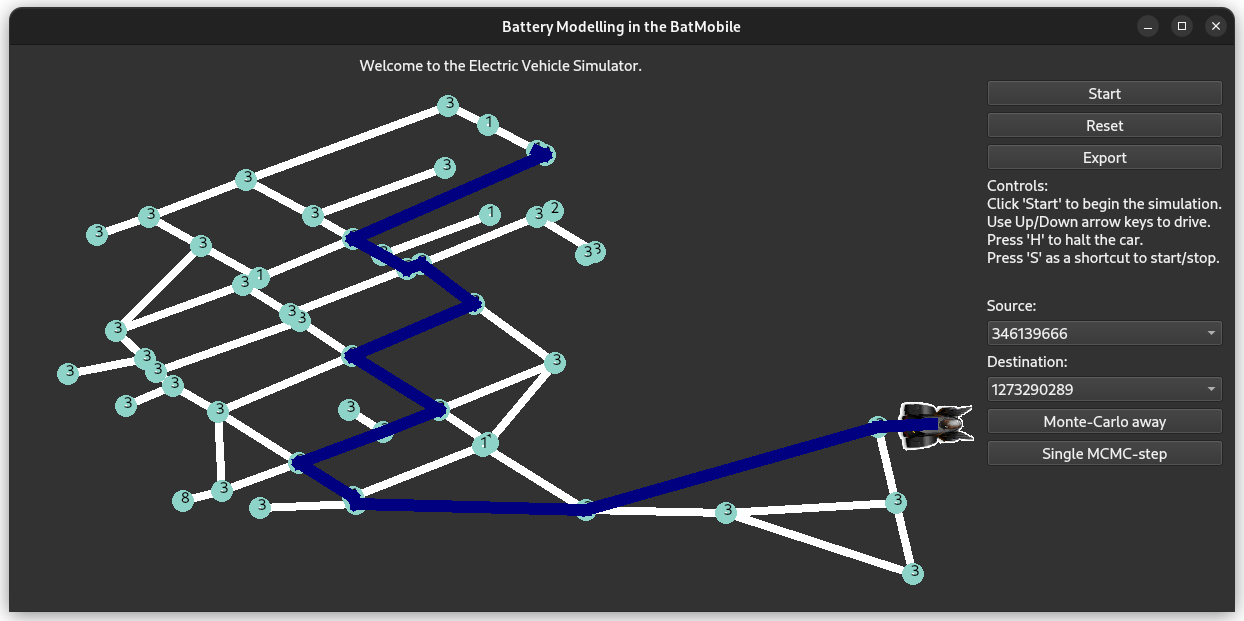
\includegraphics[width=.5\linewidth]{figures/route4.png}}\par
    \caption{Routes on the extended user interface including $A^*$ route finding along with the Monte-Carlo route perturbation-based optimisation functionality. The user can select a source and target vertex on the road graph $G = (V_G, E)$ loaded from \gls{osm} and start the optimisation procedure. The displayed road network is that of Jericho, Oxford, Oxfordshire.}
    \label{fig:perturbations}
  \end{figure}

  As a small demonstration of the procedure behind the route finding algorithm, consider \Cref{fig:jericho,fig:perturbations} which were obtained by running \\
  \centerline{\mintinline{bash}{./main.py --locality "Jericho, Oxford"}}
  where \textit{Jericho, Oxford} can of course be replaced with any locality known to \gls{osm} as data is fetched on the spot.
  \Cref{fig:perturbations} depicts the perturbations that were made in between iterations and subsequently simulated using the car and battery simulator described in \Cref{sec:simulator}.

  \section{Conclusion}
  \label{sec:discussion}
  In this report, we introduced a battery model based on the Thevenin \gls{ecm} (\Cref{fig:ecm}) which we equipped with adaptive parameters based on real-world data from a Panasonic battery product.
  We also discussed aging of the battery and how to model it effectively.

  The battery model laid the foundation for the discussion of a route finding problem on real-world road networks, which we tackled by finding the shortest route using the $A^*$-algorithm and then optimising from there using a Monte-Carlo method.

  Potential improvements are, for instance, including temperature in the discussion of aging, or using analytical methods to obtain solutions of the variational optimisation problem described in \Cref{sec:problem}.
  Namely, one could turn the optimal driving behaviour determination into a subproblem to be solved using a fully developed, deterministic spectral method in between iterations of \gls{mcmc}.
  Its optimisation routine could be significantly improved by further extending it with, for instance, Simulated Annealing, where the transition probabilities reduce over the runtime of the algorithm, slowly closing in on an optimum.
  One could even come up with a context-independent approximant for battery usage across every edge of the graph and then use this information in combination with the heuristic for the $A^*$-algorithm.

  While this paper may cover a lot of definitions and introductions, many of these can be simplified away later on and brought back into consideration when necessary.

  For future work, an even more sophisticated model could introduce the effects of other drivers influencing one's own driving behaviour.
  For example, it is neither realistic to assume one can drive at their own pace (consider traffic jams for example) nor that turning takes up no time when in many cases, crossings make up for a large portion of the driving time.

  \pagebreak
  \printbibliography

  \pagebreak
  \appendix

  \section{Code Structure and Setup}
  \label{sec:code}
  The code of this group project can be found on GitHub, namely in \href{https://github.com/MrP01/BatteryModelling}{this repository}.
  To use and sustain a Python virtual environment, install
  \href{https://python-poetry.org/}{poetry}, which works with the
  \texttt{pyproject.toml} file. After installing poetry (and subsequently
  after pulling, each time), run
  \mintinline{bash}{poetry install}
  in the project folder. To install PyBamm as well (which has $\mathcal{O}(\frac{1}{\epsilon})$ number of dependencies), run
  \mintinline{bash}{poetry install --with=pybamm}
  instead or additionally. This sadly requires Python 3.8 based on a
  pybamm restriction. Without pybamm, 3.11 should be fine too.
  Having all dependencies installed, the main interface may be launched up
  by executing \mintinline{bash}{./main.py --locality "Jericho, Oxford"}
  which starts a graphical user interface. Note that you may need to install some Qt6 dependencies.

  The relevant code structure is:

  \begin{itemize}
    \tightlist
    \item
          The folder \texttt{simulator/} is responsible for the (numerical)
          simulation itself, which may be invoked without any interface at all.

          \begin{itemize}
            \tightlist
            \item
                  \texttt{simulation.py} features the Simulation class with an
                  \texttt{iterate()} method that represents a numerical integration
                  step in time by an amount of \texttt{dt}.
            \item
                  \texttt{batgraph.py} exports a class \texttt{BatGraph} that
                  represents a graph (a tuple of sets of edges and vertices) that the
                  car will drive on.
            \item
                  \texttt{batmobile.py} contains the \texttt{BatMobile} class that
                  represents our battery mobile i.e.~car. \textbf{The vehicle simulation takes place in this file!}
            \item
                  \texttt{battery.py} is the central file for our battery modelling
                  project, which exports a \texttt{Battery} class, also featuring an
                  \texttt{iterate()} method. \textbf{Most of the battery simulation
                    takes place in this file!}
            \item
                  \texttt{optimiser.py} takes care of the optimisation part of the routing problem. It implements the Metropolis-Hastings (\gls{mcmc}) method and defines the graph perturbations.
          \end{itemize}
    \item
          The interface code is contained within the \texttt{interface/} folder.

          \begin{itemize}
            \tightlist
            \item
                  \texttt{mainwindow.py} defines the general layout and actions in the
                  user interface.
            \item
                  \texttt{batmap.py} exports the central widget that renders /
                  animates the BatMobile car on the BatGraph.
            \item
                  \texttt{graphs.py} handles the connection of the interface and (live) plots. The plots are handled by \texttt{matplotlib}.
          \end{itemize}
    \item
          \texttt{main.py} creates a \texttt{MainWindow} and runs the simulator
          GUI.
  \end{itemize}

  \section{Graph Perturbation}
  The graph perturbations described above for the \gls{mcmc} optimisation routine are implemented in \texttt{simulator/batgraph.py}. For reference, this is the relevant part of the code for perturbation and subsequent optimisation:

  \begin{minted}{python}
def airlineDistance(self, A, B):
    """Returns airline length (heuristic) between A and B."""
    dx = self.nodes[A]["x"] - self.nodes[B]["x"]
    dy = self.nodes[A]["y"] - self.nodes[B]["y"]
    return math.hypot(dx, dy)

def findShortestPath(self, source, destination) -> tuple:
    """Determine the literal shortest path from source to target, in terms of length."""
    return tuple(shortest_paths.astar_path(self, source, destination, heuristic=self.airlineDistance))

def perturbRoute(self, route: tuple) -> tuple:
    """Return a type-1, type-2 or type-3 perturbation of a given path.
    type-1: turn one edge into two edges -> route length increases by one.
    type-2: replace one node along the route with another adjacent one -> route length stays the same.
    type-3: the destination becomes part of the perturbation (shortened route).
    type-4: take a larger detour using a simple path
    """
    i = random.randrange(0, len(route))
    j = random.choice([x for x in (i + 1, i + 2, i + 3, i + 4, i - 1, i - 2, i - 3, i - 4) if 0 <= x < len(route)])
    indexA, indexB = min(i, j), max(i, j)
    nodeA, nodeB = route[indexA], route[indexB]
    if indexB - indexA <= 2:
        # type-1-2-3 perturbation:
        sharedNeighbours = set(self.neighbors(nodeA)).intersection(self.neighbors(nodeB))
        if indexB - indexA == 2:  # type-2 perturbation
            inbetween = route[indexA + 1]
            sharedNeighbours.remove(inbetween)  # ignore the element that is already part of the route
        middle = sharedNeighbours.pop()
        if middle == route[-1]:  # type-3 perturbation, destination is perturbed in
            return route[: indexA + 1] + (middle,)  # so ignore the remaining route (which will be a loop)
        return route[: indexA + 1] + (middle,) + route[indexB:]  # choose any shared neighboudan
    else:
        # type-4 perturbation:
        generator = networkx.all_simple_paths(self, nodeA, nodeB)
        return route[:indexA] + tuple(next(generator)) + route[indexB + 1 :]
  \end{minted}

  \printnoidxglossary[type=acronym, title={Acronyms}]
\end{document}
